\documentclass[10pt,a4paper,english]{article}
\usepackage{babel}
\usepackage{listings}
 \lstset{showspaces=false,
  showtabs=false,
  breaklines=true,
  showstringspaces=false,
  breakatwhitespace=true,
  commentstyle=\color{blue},
  keywordstyle=\color{orange},
  stringstyle=\color{yellow},
  basicstyle=\ttfamily,
  moredelim=[il][\textcolor{grey}]{$$},
  morekeywords=\textcolor{orange}]{yield},
  moredelim=[is][\textcolor{grey}]{\%\%}{\%\%}}
\usepackage{ae}
\usepackage{tikz}
\usetikzlibrary{positioning,matrix,shapes.arrows}
% setup tikz
\tikzset{
  modulematrix/.style={draw=blue!50!red,rounded corners,matrix of nodes,row sep=1cm,column sep=1cm,nodes={draw=green!70,align=center,font=\sffamily},inner ysep=0.5cm},
  module/.style={rounded corners, align=center, font=\sffamily, thick},
  simple module/.style={module, top color=blue!10, bottom color=blue!35, draw=blue!75, text width=40mm, minimum height=15mm},
  module down arrow/.style={module arrow, shape border rotate=-90},
  module right arrow/.style={module arrow},
module arrow/.style={single arrow, single arrow head extend=2.5mm, draw=gray!75, inner color=gray!20, outer color=gray!35, thick, shape border uses incircle, anchor=tail,minimum height=0.7cm},
}% end setup tikz
\usepackage{aeguill}
\usepackage{shortvrb}
\usepackage[latin1]{inputenc}
\usepackage{tabularx}
\usepackage{longtable}
\setlength{\extrarowheight}{2pt}
\usepackage{amsmath}
\usepackage{graphicx}
\usepackage{color}
\usepackage[dvipsnames]{xcolor}
\usepackage{multirow}
\usepackage{multicol}
\usepackage{ifthen}
\usepackage[colorlinks=true,linkcolor=blue,urlcolor=cyan]{hyperref}
\usepackage[DIV12]{typearea}
%% generator Docutils: http://docutils.sourceforge.net/
\newlength{\admonitionwidth}
\setlength{\admonitionwidth}{0.9\textwidth}
\newlength{\docinfowidth}
\setlength{\docinfowidth}{0.9\textwidth}
\newlength{\locallinewidth}
\newcommand{\optionlistlabel}[1]{\bf #1 \hfill}
\newenvironment{optionlist}[1]
{\begin{list}{}
  {\setlength{\labelwidth}{#1}
   \setlength{\rightmargin}{1cm}
   \setlength{\leftmargin}{\rightmargin}
   \addtolength{\leftmargin}{\labelwidth}
   \addtolength{\leftmargin}{\labelsep}
   \renewcommand{\makelabel}{\optionlistlabel}}
}{\end{list}}
\newlength{\lineblockindentation}
\setlength{\lineblockindentation}{2.5em}
\newenvironment{lineblock}[1]
{\begin{list}{}
  {\setlength{\partopsep}{\parskip}
   \addtolength{\partopsep}{\baselineskip}
   \topsep0pt\itemsep0.15\baselineskip\parsep0pt
   \leftmargin#1}
 \raggedright}
{\end{list}}
% begin: floats for footnotes tweaking.
\setlength{\floatsep}{0.5em}
\setlength{\textfloatsep}{\fill}
\addtolength{\textfloatsep}{3em}
%__________________________________________________________________________________
\newcommand{\code}[1]{{\tt{\textit{#1}}}}
\renewcommand{\textfraction}{0.5}
\renewcommand{\topfraction}{0.5}
\renewcommand{\bottomfraction}{0.5}
%__________________________________________________________________________________
% Chapters 
\newcounter{Chapcounter}
\newcommand\showmycounter{\addtocounter{Chapcounter}{1}\themycounter}
\newcommand{\chapter}[1] 
{ {\centering          
  \addtocounter{Chapcounter}{1} \Large \underline{\textbf{ \color{blue} Chapter \theChapcounter: ~#1}} }   
  \addcontentsline{toc}{section}{ \color{blue} Chapter:~\theChapcounter~~ #1}    
}% End Chapters
\setcounter{totalnumber}{50}
\setcounter{topnumber}{50}
\setcounter{bottomnumber}{50}
% end floats for footnotes
% some commands, that could be overwritten in the style file.
\newcommand{\rubric}[1]{\subsection*{~\hfill {\it #1} \hfill ~}}
\newcommand{\abbrhighcol}[1]{\textbf{\textit{#1}}}
\newcommand{\subtitle}[1] {\title{\abbrhighcol
                                           	{\underline{#1}}}}
	
\newcommand{\titlereference}[1]{\textsl{#1}}
% end of "some commands"
\title{Testing is a MUST \newline Version 0.8}

\author{Harald Glab-Plhak{\textless}\href{mailto:hglabplhak@icloud.com}{hglabplhak@icloud.com}{\textgreater}}
\date{\today{}}
%______________________________________________________________________________________
\hypersetup{
pdftitle={Testing is a MUST Version 0.8}, 
pdfauthor={Harald Glab-Plhak (staatl.gepr. Inf) {\textless}hglabplhak@icloud.com{\textgreater}}%;Mike Sperber (CEO Active Group Tübingen) {\textless}michael.sperber@active-group.de{\textgreater}}
}

%______________________________________________________________________________________
\begin{document}
%______________________________________________________________________________________

\maketitle
\subtitle{About automated test methods and more.....}
\tableofcontents

%______________________________________________________________________________________
%-1 \part{part}
%0	\chapter{chapter}
%1	\section{section}
%2	\subsection{subsection}
%3	\subsubsection{subsubsection}
%4	\paragraph{paragraph}
%5	\subparagraph{subparagraph}
\section{Information}
\label{sec:information}
\begin{flushleft}
This document and the whole project including the source code is licensed under the MIT license. The only restriction is that it MUST not be used commercial. A copy and further enhancements are allowed as long as the license and the copy right is saved. I intended that these test descriptions project is used for educational purposes. I trust in the integrity of those who use or duplicate the project and develop on this project.   
\end{flushleft}
\abbrhighcol{\textcopyright Harald Glab-Plhak 2025}
\section{Abstract}
\label{sec:abstract}
\begin{flushleft}
The target of this project is to give an overview of testing and test automation. The project also shows pitfalls and a style of development making testing and automation of tests easier. The project is made to show up how testing can be introduced in a project or product so that there is a common sense in the teams what things and processes can be useful to have a real test culture. In a world there the projects and products get more and more complex in cause of using cloud technologies, machine learning and KI as well as massive parallel execution it is also more and more necessary to develop automated tests and processes which allow us to get the complex things handled. Also the definition of test cases down to the last detail are important as well as a detailed logging of test results. These all is defined more and more detailed and there are many test-theories and project development and integration theories and practises as DevOPS with CI/CD. Here the short descriptions as footnotes taken from the KI of Google. \abbrhighcol{DevOPS}\footnote{\abbrhighcol{DevOPS: }is a set of practices and a culture that combines software Development and IT Operations to shorten the software development lifecycle and provide continuous delivery with high quality. It breaks down the traditional silos between these teams, fostering collaboration and shared responsibility to accelerate the delivery of software while improving reliability. Key practices include automation, continuous integration and delivery (CI/CD), and using tools to streamline the process from planning through deployment and monitoring.} and \abbrhighcol{CI/CD}\footnote{\abbrhighcol{CI/CD: } Continuous integration and continuous delivery (CI/CD) have revolutionized how software teams work together. Gone are the days of code integration headaches and repeated manual processes. CI/CD makes modern software development possible fast, reliable, and automated.}
. All these things are themselves very complex I try in this document to show up a path through this 'jungle' . 
\end{flushleft}
\section{Introduction}
\label{sec:introduction}
\subsection{The different Test Methods in Test automation (UNIT -Test , Functional Test, Performance Functional Test)}
\label{sec:intro}
\begin{flushleft}
In order to get the goal of a clean and correct code and functionality we must have a look on the program logic in different views. 
\end{flushleft}
\begin{itemize}
\item{We have a view where we look for a complete well defined transaction in the program and have to check wether input and output is correct. Here we use \abbrhighcol{Functional Tests}.\footnote{\abbrhighcol{Functional Tests.}: These tests to check a complete request or transaction to an application. They treat the methods called inside and the logic inside the borders of the transaction as a \abbrhighcol{BLACK BOX}. So it does not matter what the different functions classes or whatever process in what place even if the result is correct. }.}
\item{The other view is more that we look at the atomic functions processing more or less complex logic. Here we also look for input / output of the functionality in that unit but we also keep in mind the internal logic and the functions which are called before / after and / or if third-party functionality is called which can cause that we not really test our own logic / flow of control. These kind of tests are called \abbrhighcol{Unit Tests} \footnote{\abbrhighcol{Unit Tests}: Unit Tests are the tests with which small Units are tested e.g. public functions}} 
\item{And now to the last view I will mention here where are for sure many more. We have to look how high the throughput of our application must be and if we reach that goal with our logic and the fact how we realised it in detail. These are \abbrhighcol{Performance Tests}\footnote{\abbrhighcol{Performance Tests}: These tests are designed in a way that the performance of Units as well as the performance of requests and transactions or e.g. import / export in bulk can be tested} and. the best is to let them run after each change and prior deployment of each minor and major release}
\end{itemize}
\subsection{UNIT Testing in an automated environment}
\begin{flushleft}
 So now our development team coded something and the specification is clear and clean transformed to code. Ups what shall we do now ? We have to test it and it gets more and more and more. The code is for quality reasons debugged by the developers but we need something more efficient. So we search for a test-framework where we are able to define Tests for the specific functions. This test-framework can handle all these things if we use it right. The advantage of this way testing things is that the tests are coded in Python / RUST / Haskell / Java / Clojure / Racket / Scheme48 and other Scheme and LISP dialects / C / C++ and so on and executing them another time without code-change they will do the same and exactly the same. This is one problem for manual testing. The Tester is a human being and we are full of mistakes in our doing. For manual tests we have later a look on it you have to create for each test a step by step list which shows up a detailed description for each step. For \abbrhighcol{UNIT Tests} we also need a description what will happen step by step but we tell our coded test to do it for us thousands of times. Now have a closer look on UNIT Testing in Java and Clojure. For Java the most popular framework will be \abbrhighcol{JUNIT} this framework is grown to a very large extensive test environment.
 \end{flushleft}
 \chapter{An Introduction to test types and automation of tests} 
 \section{The different ways to divide tests in categories}
 \subsection{From the technical point of view}
 \begin{flushleft}
 \begin{enumerate}
\item{\abbrhighcol{Simple technical difference:}
 \begin{itemize}
 \item{\abbrhighcol{BLACK BOX Test}: This kind of test only knows about the interface to test that means the defined Input and the awaited Output}
  \item{\abbrhighcol{GREY BOX Test}: This kind of test only knows about the interface to test. and about some inside details that means the defined Input and the awaited Output with the background that some details are known. So it is something between BLACK-(GREY)-WHITE BOX. This kind of test category is found very often in reality.}
 \item{\abbrhighcol{WHITE BOX Test}: Here the test also takes care about the way the function is implemented in technical detail}
 \end{itemize}}
 \item{\abbrhighcol{UNIT Tests:} These Tests check the functionality on a level of for example public functions on an object. Functions where access can be gained only by a hack (private functions) should never be tested directly in the normal case doing this is bad style.}
 \item{\abbrhighcol{Functional Tests:} These Tests check the functionality of a greater part of. the application e.g. One specific transaction.}
 \end{enumerate}
 \end{flushleft}
 \subsection{Another way to make categories is delivery, user and release oriented}
 \begin{flushleft}
 \begin{enumerate}
\item{\abbrhighcol{Acceptance Test:} Here the project or product is tested to be informed about usability and acceptance by the user}
\item{\abbrhighcol{Regression Test:} This test is done always after one or more changes. Either in the service or its environment}
\item{\abbrhighcol{Release Test:} This tests are done for. each major or minor release. Here. the point is that it is tested if the new functionality works and if the existing things also work again. What is also tested is the migration from the old to the new release.}
\item{\abbrhighcol{Performance Tests:} In these tests the overall or partial performance is good and sufficient for the needs of the application and if e.g. a change in a function influences performance negative.}
\end{enumerate}
\end{flushleft}
\section{A example how to design and realise an automated test}
\begin{flushleft}
As an algoritmic fuction example for testing we use the widely spreaded sorting algorithm Quick-Sort. I know this is a example of a very low level functionality which is covered already in the JDK since a long time e.g. : SortedList or the sort feature in collection streaming.
But I use it because it is a simple example.
%
% code highlighting ???? // for different languages
%

\begin{lstlisting}[language=Java]
public void quickSort(int arr[], int begin,  int end) { 
   if (begin <. end) {
       int partitionIndex = partition(arr, begin, end);       
       quickSort(arr, begin, partitionIndex - 1);
       quickSort(arr, partitionIndex + 1, end); 
    } 
}
\end{lstlisting}
\abbrhighcol{HINT for beginners: to get it running you need the partition method. For the beginners this algorithm is in APENDIX II}.\newline So ok here we have now something to
test. What we need now is a testing framework containing assertion functions and annotations to annotate test methods. For this we use the most popular Java Testing framework JUNIT. The most important annotations in JUNIT are the following method annotations. The methods need to be public:
\end{flushleft}
\begin{itemize} 
\item{\abbrhighcol{@Test}: Annotate the test method as a method containing a test}
\item{\abbrhighcol{@Before}: Execute before each test}
\item{\abbrhighcol{@After}: Execute after each test}
\end{itemize}
Here first a example of a very tiny test:

\begin{lstlisting}[language=Java]
@Test
public void simpleQSortTest() {
		Integer[] theArrayToSort = {6, 7, 4, 2, 78, 45 ,1 ,5, 15};
		Integer[] expectedSorted = {1, 2, 4, 5, 6, 7, 15, 45, 78};
		quickSort(theArrayToSort, 0, (arrayToSort.length - 1));
		assertThat(arrayToSort, is(expectedSorted)); // if this assert fails quicksort does not
// work correctly
}
\end{lstlisting}
Here in this test the easiest case is tested. It is tested if the array given is sorted after quicksort. The other cases like given wrong data by type e.g. Strings instead of Integer are not tested. In our case this won't work because the whole thing won't even compile in that case. So to show how such a Test will work let us elaborate the whole function a bit.
Here is our new function which is much more flexible :
\begin{lstlisting}[language=Java]
public class QBubbleMerge<T> {
    private QBubbleMerge() {
    }

    public static Integer[] quickSort(Integer[] arr, SortDirection direction, Integer begin, Integer end) {
        int partitionIndex = partition(arr, direction, begin, end);
        quickSort(arr, direction, begin, partitionIndex - 1);
        quickSort(arr, direction, partitionIndex + 1, end);
        return arr;
    }

    private static Integer partition(Integer[] arr, SortDirection direction, Integer begin, Integer end) {
        int pivot = arr[end];
        int i = begin - 1;

        for(int j = begin; j < end; ++j) {
            Boolean swapit = Boolean.FALSE;
            switch (direction.ordinal()) {
                case 0 -> swapit = Boolean.FALSE;
                case 1 -> swapit = arr[j].compareTo(pivot) >= 0;
                case 2 -> swapit = arr[j].compareTo(pivot) <= 0;
            }

            if (swapit) {
                ++i;
                Integer swapTemp = arr[i + 1];
                arr[i + 1] = arr[end];
                arr[end] = swapTemp;
                return i + 1;
            }

            Integer swapTemp = arr[i];
            arr[i] = arr[j];
            arr[j] = swapTemp;
        }

        ++i;
        return i;
    }

    public static void main(String[] args) {
        quickSort(SortData.SORT_DATA, QBubbleMerge.SortDirection.DESC, 0, SortData.SORT_DATA.length);
        quickSort(SortData.SORT_DATA, QBubbleMerge.SortDirection.ASC, 0, SortData.SORT_DATA.length);
    }

    public static enum SortDirection {
        DEFAULT,
        DESC,
        ASC;
    }
}
\end{lstlisting}
\subsection{And here are a few tests for it to see how UNIT Testing works:}
Here are a scelleton how to test the UNIT with JUNIT in Java (The code will be discussed in the next chapters / sections):
\begin{lstlisting}[language=Java]
package io.examples.sort;


import org.junit.jupiter.api.BeforeAll;
import org.junit.jupiter.api.BeforeEach;
import org.junit.jupiter.api.Test;

public class QBubbleMergeTest {

    private QBubbleMergeTest() {

    }

    @BeforeAll
    public static void beforeAll() {

    }


    @BeforeEach
    public void beforeEach() {

    }


    @Test
    public void testQuickSortSimple() {

    }

    @Test
    public void testBubbleSortSimple() {

    }

    @Test
    public void testMergeSortSimple() {
    
    }
 \end{lstlisting}
 \subsection{First Resume}
\begin{flushleft}
Ok now we have some Tests checking random some aspects. To get a real good coverage when testing a function we first have to know it's specification that means what is the input and what is the output of a function we test. We also have to know what happens in the function when processing the input to get either the valid output or a clear error which really explains what is missing or wrong. The more parameters we have the more the complexity tests for the function grows. If we when have a function with 5 parameters and each parameter has 15 combinations of values (The parameter may be an Object reference) we get a exponential growth of possibilities what would went wrong.\newline\newline The main error by people who have less experience in Testing is to check the parameters together only  in one test function. \abbrhighcol{THIS IS A NOT TO DO!!!!}. A better way is to make a test for each parameter. \newline\newline To get the complexity broken down we should make tests where 4 parameters are in a good range and only one is out of range or has a value which does not fit the four others parameters values. So you might argue what is with the combination where two parameters or three parameters have values which do not fit in combination. For this cases we can write some generic tests which walk via recursion through each valid combination. But do not test the case in that way where one or two parameters have a value out of their range which is defined by the functionality and which values and combination of values the function covers. Even if you plan to do test driven development this kind of proceeding gets more important for otherwise you do not know in the end in which case and why the function fails. To be sure all works you have to write \abbrhighcol{UNIT Tests}for each public method in each class. \newline The private methods are tested indirect. A bad style is (with only a very very few exceptions - should never happen) to access private functions for the reason of testing them via privileged access. \newline Ok this works in Java up to 1.8. But one thing has to be clear:\abbrhighcol{For making good functional unit or other testing in a proper way it should never be necessary to use algorithms which break the normal ways of coding. No good developer will design a program and the time he is ready use a function which accesses another function which is e.g. private and the language is not designed to do it in that way.} \newline If you see such code begin looking at the design of this part delete the code and rewrite it completely following the design in a clean way. Why write it completely new. One reason is if you do after these functions are written test driven development for some parts such parts will lead you off the road of a clean design.
\end{flushleft}
\section{How to design Automated Functional Tests}
\begin{flushleft}
\end{flushleft}
\subsection{The Basics}
\begin{flushleft}
For the automated Functional Testing we can set up a environment with e.g. at least \abbrhighcol{JUNIT}. Now you may think JUNIT is only for Unit testing
But for sure we can use it because the things we call inside a test are flexible.
Now we do not call functions inside the Test but we call for example our WebService Application and check the HTTP and extended Result given by the response data for example JSON in a RESTful service call.\newline In functional testing we have actively to forget about the implementation details only the interfaces like WebServices count. The input has to
be defined and the output for each input has to be known. The thing between both is in Functional Testing a big black box. This are the basics. The setup for a Functional Testing is dependent on the application we have.
\end{flushleft}
\section{Performance Testing}
\begin{flushleft}
Looking at the performance testing it gets a bit more tricky.
For getting a real good Performance Testing we have to look at the System in at least two different ways:
\end{flushleft}
\begin{enumerate}
\item{Looking at specific functionality:
\begin{itemize}
\item{When looking at specific functionality like database access in bulk or at archiving large files or many files it is not so hard. We have to set up the system in a way that the factors which disturb the running test are minimised. The advantage is we see how performant this special features are if no other things are kept in mind and no other functionality like background jobs etc. is configured. The disadvantage is that we look at the functionality in some kind of a bubble ;-)} 
\item{Ok now we can set up the system if we look at file archiving with the specific archiving method (SFTP , Local Storage, Cloud Storage....) exactly for this style and method of archiving. We can then use a Testing Tool like e.g. Grafana ... There are many testing tools configurable in a way that the requests can be fired in milliseconds to a WebApplication as example.}
\item{It is common sense if you look e.g. on archiving to test the same scenario with the same document count and document size with the different archiving methods so that the whole thing gets 1:1 comparable}
\end{itemize}}
\item{Looking at the System as a complex with many functions run in parallel and may be also on different Nodes / partly in a cloud and so on:
\begin{itemize}
\item{If twe look at the system in that way we have to check and look how our system is most commonly used by the customer. In this way then the system is configured. May be with other long running background Jobs or Archive Hooks or other Extensions as for example encrypt data immediately at the point reading it.}
\item{The system setup is n the best case automised may be via DevOPS.}
\item{Here it is also I think the best idea if you test different archive drivers to use comparable Sizes of Documents and the same count of documents as well as in this case the file type off the document playing a role if it is not pure I/O.}
\end{itemize}}
\end{enumerate}
\begin{flushleft}
The first thing necessary for each way of performance testing is to be able to run the application on a dedicated machine or cluster to be sure that no other application which is not in connection with the application we test wastes the resources used for the test. The second thing is to do the tests in a way with different set ups but with a comparable amount and size of data. The other thing is that in both scenarios the decision at which point the measuring takes place is essential this is nearly the greatest issue something potentially can went wrong so that there is nothing (no value) which tells you that the system is really performant.
\end{flushleft}
\section{Release Testing}
- In the main sense release testing is a kind of testing looking at the complete system the new and old features. The changes / enhancements for configuration and database set up as well as the test if the whole thing can be migrated in acceptable time and in a way the system of the customer is not corrupted
- One other thing which has to be tested for each feature is the backward compatibility in each way because no customer will accept it when he has also to migrate all the other elder services he uses since years with success.  For release testing the following tests must take place.
\subsection{Installation / Integration / Migration Testing}
\begin{enumerate}
\item{Test the installation for the standard way and in the way how the most customers use the system. After that test the installation of each extension which may exist and the other different settings}
\item{Dependent on the License model you use you also have to test the different configurations of your license model}
\item{The Integration test on the other side includes also the most common settings in connection to other modules or applications running on the system.}
\item{The migration test is in the main thing a test which checks if database and configuration migration scripts do what they have to do and if migration is really possible or if something is broken so especially the migration test is part of the release test but it won't be a mistake not to run it the first time with the publication of a new release to avoid such mistakes prior and have more time to fix it if something went wrong.}
\end{enumerate}
\subsection{Regression Testing}
\begin{enumerate}
\item{The regression test is a test which is made in periods for the running system instances in the best case for each used customer setup. This test ensures that the system runs without problems even though the services and OS versions or VM versions changed.}
\item{Continuously testing means the incremental testing during development. For this tests the automated way of testing is always the best option because no developer would have the time to test all these things manually. One exception here is the test of things which include the GUI. Up to now I do not know any framework for automated GUI testing which is running without having a great effort in the setup of the tool.}
\end{enumerate}
\section{An example for our scenario}
\begin{flushleft}
Think about the following Rest Service:
\end{flushleft}
\begin{itemize}
\item{We have a service call to create documents}
\item{We have a service call to update documents}
\item{We have a service call to get / query documents}
\item{We have a service call to delete documents}
\end{itemize}
\begin{flushleft}
Our Application implements this call in a Apache Tomcat with a database in background and a SFTP archive (Azure, Hitachi, Hadoop, Centera will be also used in real world even today but this is for our example to complex due to the neccessary setup for this storage solutions.
\end{flushleft}
\subsection{The Development / Test Environment}
\begin{itemize}
\item{Source Control e.g. BItBucket}
\item{Project Task/Requirements Management e.g. Jira}
\item{Runtime Environment e.g. Docker}
\item{Runner for tests e.g. Jenkins}
\item{Running Docker Remote e.g. Portainer}
\item{JUNIT Styled and Based TestLauncher Proprietary developed Test Runner.  Now we can think about how to set up and run the whole thing. NO at first we have to define the Test Cases. Because we need this cases to decide how this test cases can be run . Some cases are really good for automation and other need manual testing}
\end{itemize}
\subsection{Test case definition cookbook}
\begin{flushleft}
To write test cases whith a good coverage of the system requirements is the most difficult thing in doing good testing for functionality performance setup and so on.
Now as example we use a functionality:The user likes to store a document / encrypt / sign it and make sure thata legal hold can be set for the document. In addition he needs by the law a retzention time of 10 y for the document in this time the document has to be protected from deletion. During the whole time irt has to be impossible to change the document. What he gets as input is the document in paper form.
\end{flushleft}
We need the complete specification for the functionality:
Workflow: Store Business Document
Description: The customer likes to save a document which arrives in paper form inn a way 
that it is signed encrypted and has a retention time of 10 years (type: UN\_DELETEABLE READONLY)
\begin{enumerate}
\item{The document has to be scanned and the scan result has to be put to the incoming document stack storage. To ensure the document is good for long term archiving we use the file format PDF and to be sure the sub-form PDF/A - the /A stands for archive}
\item{For storing the document the service grabs the document from stack stores into a long term archive system (in our case \abbrhighcol{Centera}\footnote{\abbrhighcol{Centera}: Centera is a hard and software for archiving documents in \abbrhighcol{BLOBS} identified by a key.}) and sets the \abbrhighcol{ARCHIVED} flag}
\item{The document is encrypted and signed in the same step it is read by the application this is done by using special data-streams like they exist e.g. in the IAIK framework or in BouncyCastle}
\item{Signing parameters are EC (Eliptic Curve) with the strongest usual encryption depth.}
\item{The encryption is done by CMS (Crypted Message Syntax) Envelop}
\item{Now to make a change much more difficult the document gets a hash value with strength 512 which is stored in a document hash tree}
\item{Our retention management that there is a new document with the retention 10 years DO\_NOT\_DELETE after (10 years + 1 day) ERASE}
\item{Now after the retention mark is set we set the document capable for a possible legal hold}
\item{Now all things are committed and the transaction of saving a document is completed} 
\end{enumerate}
Oh nice we have only nine steps to test what a luck.Oh dear don't be happy to early in each step I see without analysing it step by step about 5 test cases. Starting at data transfer. The different returns a scan can deliver nd the document conversion to PDF/A. Oh we are talking about the first step and we do not have analyzed each parameter which can be wrong yet.
How to analyze the steps:
Let us take as example step 4 and 5 because testing encryption and. hash values is very funny ;-).
\begin{itemize}
\item{Step 4: Check the configuration (Hash Tree strength, Algorithm Type , Strength, Provider (e.g. IAIK correctly configured ? ) so break it down
\begin{enumerate}
\item{call get-crypto-conf}
\item{ the crypto provider config - check initialisation result code}
\item{ check if hash-tree generation is turned on}
\item{check if signing is on}
\item{ check if encrypt is on}
\item{check the hash tree digest strength}
\item{check if signing algorithm is correct}
\item{check if the value for the encryption algorithm is ok}
\end{enumerate}}
\item{Step 5: Check the outcome and incoming data before and after sign / encrypt:
\begin{enumerate}
\item{Check if the document is a real PDF/A}
\item{run the Sign/Encrypt view the outcome}
\item{decrypt the document look if outcome is a correctly signed document}
\item{check the signature via verification e.g. by using DSS-ESIG (Electronic European Standardised Signing and encrypting) as well as signature and document verification.}
\item{now check if the document is found in the HashTree check the Hash value and Strength}
\end{enumerate}}
\end{itemize}
And now you see two steps and so much to check. Hope I have not forgot something
Now you can take this defines steps think about how this steps and actions are triggered in the application and what kind of matcher checks you need to do the test automated.
  


\section{ANOTHER POINT WHY NOT TESTS FIRST \-\> Test Driven Development}
\subsection{Test driven development a short view.}
 The idea behind Test Driven Development is that of course tests are very important to the quality and the comfort of a software. The method is not very old. In former times there was a running gag in the community of developers: Testing is something for cowards. 
Nowadays it is clear that the software gets more and more flexible and complex, The fact that most things run in parallel and there it is possible in cloud solutions is another reason to test software very intensive for being sure that the software is running even if there are maybe 40 tasks running in parallel mode.This leads to the conclusion that a software without tests will get useless.Now one had the idea that the interfaces are one of the most important thing which ensures that the design is clear and clean, To get the coders , designers and all the ones who deal with the code in a mode of being forced to develop in a way that at first the interface has to be designed in a way all fits together the idea of writing tests (at first with empty stubs which define the interfaces and see if all things will work interlocked that means the return of the last step is exactly the thing the next step needs and defines.
And so the Test Driven Development was born.
\subsection{How to realise this thoughts}
To realise this thougts we have today test frameworks like **JUNIT** in Java or simply **deftest** in Clojure. Inside the different test methods which we are able to define in **JUNIT** with the **@Test** annotation the logic can be designed and here there are also the asserts if the last call was successful and delivers the correct input for the following task.\subsection{Example of such a test in Java}
\begin{lstlisting}[language=Java]
public class ATest extends BaseOfTests {

private Integer derfault = 110;
 /* CTOR*/
 public ATest() {
}

@Test
public aSpecificTest () 
{

		Integer result = myFirstMethod(this.default); /*here it seems that there is a addition of 86,,, but what the function does really is hidden for us and for sure in the beginning it's empty*/
		String resultStr =  mySecondMethod (result);
  		assertThat(resultString is("196"));
}
}
\end{lstlisting}
And out of these tests stubs for the interface are created

\begin{lstlisting}[language=Java]
public interface MyAppIfc {

	public Integer myFirstMethod (Integer input);

	public String mySecondMethod (Integer toConvert);
}
\end{lstlisting}

And the class implementing our great highly sophisticated interface ;-) may be look
as follows


\begin{lstlisting}[language=Java]
public class MyRealApp implements MyAppIfc {

	@Override
	public Integer myFirstMethod (Integer input) {
			Integer result = (input + 86);
			return result;	
	}
	
	@Override
	public String mySecondMethod (Integer input) {
		return Integer.toString(input);
	}
}}
\end{lstlisting}
\begin{flushleft}
And now we can test the thing out of the box for the test is already there.
\end{flushleft}
\chapter{Test driven development}
\section{Short introduction}
After that we can think about how test driven development can be used to have a well defined interface and to code a application. Test driven development is a kind of development where we define in opposite to the prior example the tests first. Test driven development has the advantage that we see immediately if the function we designed works like it should work because the test shows already up the call and return value of a function how we designed it. Instead of adapting the test to our functionality we write the functionality in the way that we have a test first written according to the requirement.\newline
\section{Make the proof of concept}
To show how test driven development can be done in a project we make a tiny project called 'Calculator' this calculator is a calculator for mathematical expressions with a GUI. The project is defined in Java with a numeric tower and SWING as graphical interface. Here first the tests are defined and after that the functions are implemented. After done so there are Functional Tests and defined Interactive Tests.
\newpage
\subsection{How to do Test Driven Development - Diagram}
\abbrhighcol{Example with Java and IntelliJ / Maven}
\begin{flushleft}

\end{flushleft}
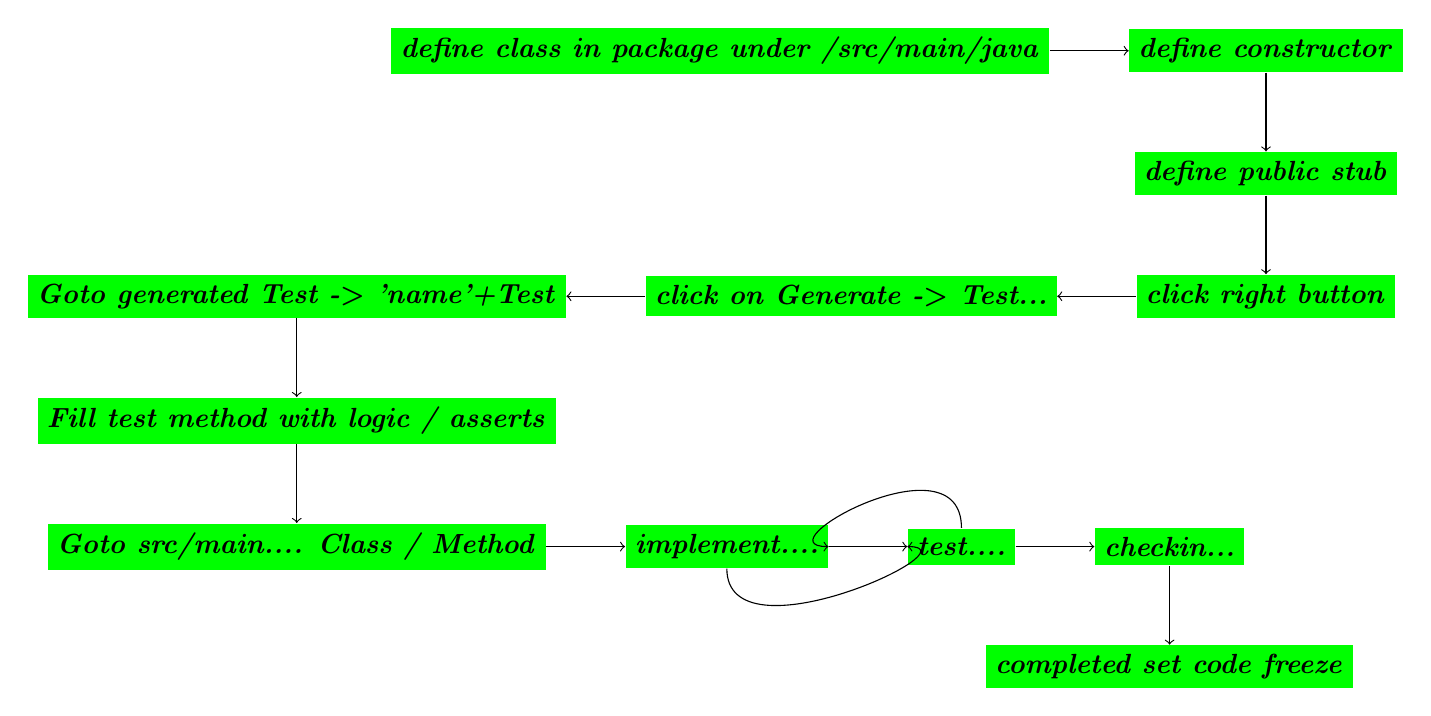
\begin{tikzpicture}
%the nodes of the snake
\node [fill=green] (start) {\abbrhighcol{define class in package under /src/main/java}}; 
\node [fill=green,right=of  start] (next1) {\abbrhighcol{define constructor}};
\node [fill=green,below=of  next1] (next2) {\abbrhighcol{define public stub}};
\node [fill=green,below=of  next2] (next3) {\abbrhighcol{click right button}};
\node [fill=green,left=of  next3] (next4) {\abbrhighcol{click on Generate -> Test...}};
\node [fill=green,left=of  next4] (next5) {\abbrhighcol{Goto generated Test -> 'name'+Test}};
\node [fill=green,below=of  next5] (next6) {\abbrhighcol{Fill test method with logic / asserts}};
\node [fill=green,below=of  next6] (next7) {\abbrhighcol{Goto src/main.... Class / Method}};
\node [fill=green,right=of  next7] (next8) {\abbrhighcol{implement....}};
\node [fill=green,right=of  next8] (next9) {\abbrhighcol{test....}};
\node [fill=green,right=of  next9] (next10) {\abbrhighcol{checkin...}};
\node [fill=green,below=of  next10] (next11) {\abbrhighcol{completed set code freeze}};
;%drawings of lines for the snake
\draw[->] (start.east) -- (next1.west);

\draw[->] (next1.south) -- (next2.north);

\draw[->] (next2.south) -- (next3.north);

\draw[->] (next3.west) -- (next4.east);

\draw[->] (next4.west) -- (next5.east);

\draw[->] (next5.south) -- (next6.north);

\draw[->] (next6.south) -- (next7.north);

\draw[->] (next7.east) -- (next8.west);

\draw[->] (next8.east) -- (next9.west);

\draw[->] (next8.south) .. controls +(down:12mm) and +(right:9mm) .. (next9.west);

\draw[->] (next9.north) .. controls +(up:12mm) and +(left:9mm) .. (next8.east);

\draw[->] (next9.east) -- (next10.west);

\draw[->] (next10.south) -- (next11.north);

\end{tikzpicture}

\subsection{How to do Test Driven Development - Step by Step Description}
\abbrhighcol{Example with Java and IntelliJ / Maven}
\begin{enumerate}
\item{\abbrhighcol{define class in package under /src/main/java} -> usually we start with any kind of new code in our case here we define a new class.}
\item{\abbrhighcol{define constructor} -> technical necessary...}
\item{\abbrhighcol{define public stub} -> this stub defines the interface with parameters and return value.}
\item{\abbrhighcol{click right button} -> IntelliJ specific...}
\item{\abbrhighcol{click on Generate -> Test...} Now a new test class is defined in src/test/java/'package' with the name of the class to test and the suffix test.}
\item{\abbrhighcol{Goto generated Test -> 'name'+Test} -> now we define tests for our stub according to the requirements.}
\item{\abbrhighcol{Fill test method with logic / asserts}-> we have to take care that the asserts and the test logic is clean and proper and reflects the requirements 100\%.}
\item{\abbrhighcol{Goto src/main.... Class / Method}-> now we go back to the implementation}
\item{\abbrhighcol{implement....} -> implement and go to test.}
\item{\abbrhighcol{test....} -> test the implementation and if necessary refine the tests. If all is ok go to the next step if not go back.}
\item{\abbrhighcol{checkin....} -> in this step we checkin the code and the tests. The checkin must be at least compilable.}
\item{\abbrhighcol{completed set code freeze} -> now we declare the task as ready but if a code review shows errors or unclean code it may be re-opened.}
\end{enumerate}
\subsection{See how this works in our example with the calculator}
\chapter{The test types in detail}
\begin{flushleft}
For the test types you will see there are different ways of categorisation. I will show them without telling the one or the other way is better, because in each discipline of data and computer science there are always different ways of thinking. Here is the categorisation we had in my former company:
\abbrhighcol{Functional Testing} checks if the entire system works as intended, while \abbrhighcol{Unit Testing} ensures individual code components function correctly. Scope: Functional Testing evaluates entire workflows and features, whereas Unit Testing isolates and tests specific functions or code segments.\newline
\abbrhighcol{REMARK:}\textit{For the other categorising and describing the alternate test types I used also input from} \hyperref[ref:references]{Solutions Hub -- see web link(1.)}
\end{flushleft}
\section{Test types in overview often used}
\begin{flushleft}
Here at first the part how many companies define the different test:\newline
There is a separation between the tests in a way that the test types are divided by defining UNIT Testing which is a kind of White Box test designed and executed by the developer. For very important UNIT tests some Jenkins-Test Jobs can be defined. The other Tests are Black Box Tests as Functional Tests, Performance Tests, Stress Tests and so on. For these tests it is good to define Jenkins-Test-Jobs with these defined Jobs also Regression and RE-Testing can be done.
\end{flushleft}
\subsection{Black Box testing type}
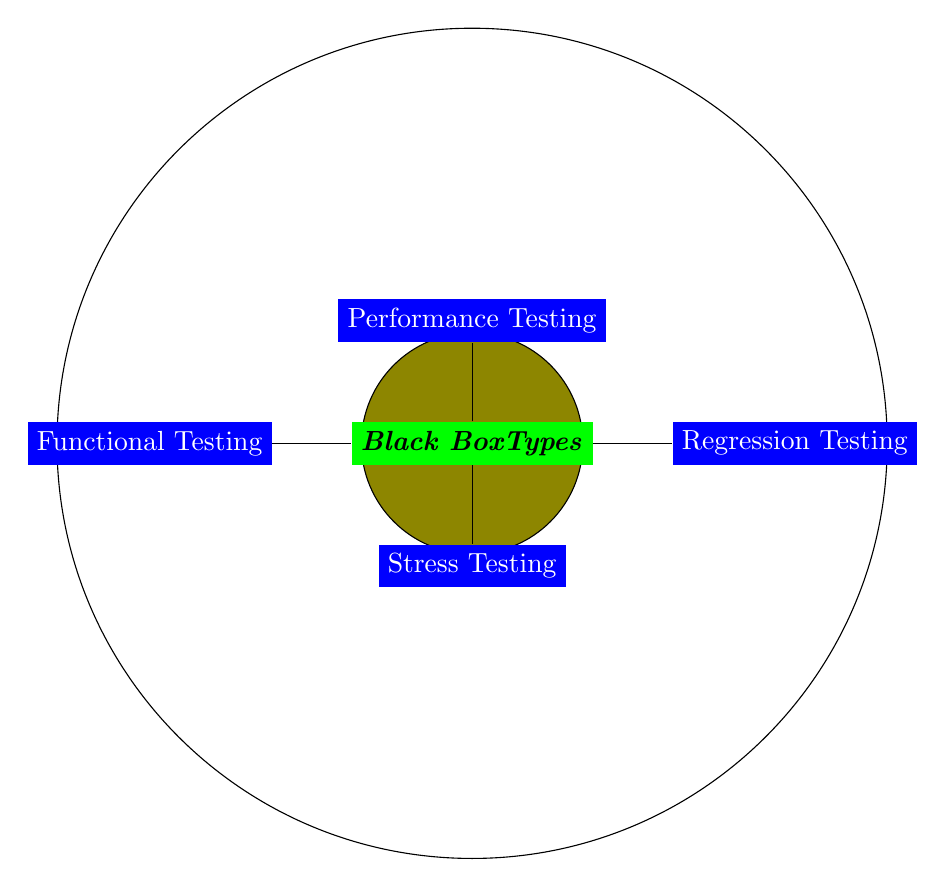
\begin{tikzpicture}
%% fun tests circle
\draw  [fill=white](0,0) circle  (150pt);
\draw  [fill=olive](0,0) circle  (40pt);
%the nodes
\node [fill=green] (blackCenter) {\abbrhighcol{Black Box \newline Types}};
\node [fill=blue,left=of  blackCenter] (blackLeft) {\color{white}Functional Testing};
\node [fill=blue,right=of blackCenter] (blackRight) {\color{white}Regression Testing};
\node [fill=blue,above=of  blackCenter] (blackAbove) {\color{white}Performance Testing};
\node [fill=blue,below=of blackCenter] (blackBelow) {\color{white}Stress Testing};
%drawings of lines
\draw[-] (blackCenter.west) -- (blackLeft.east);
\draw[-] (blackCenter.east) -- (blackRight.west);

\draw[-] (blackCenter.north) -- (blackAbove.south);
\draw[-] (blackCenter.south) -- (blackBelow.north);

\end{tikzpicture}
\subsection{White box testing type}
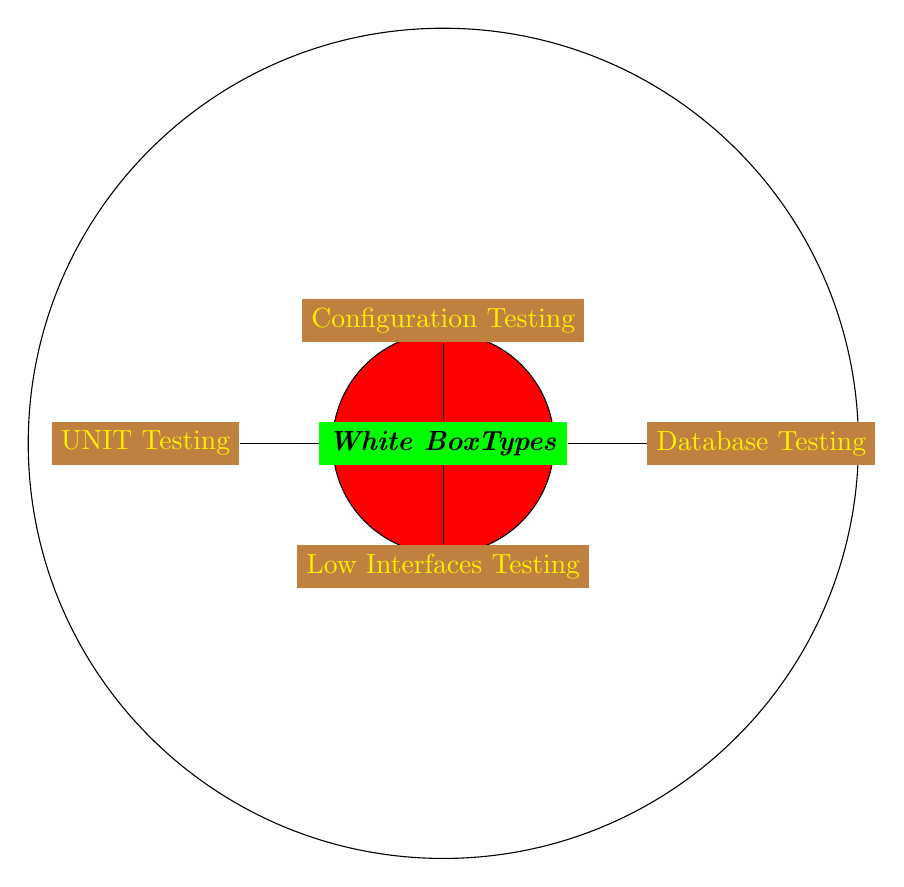
\begin{tikzpicture}
%% fun tests circle
\draw  [fill=white](0,0) circle  (150pt);
\draw  [fill=red](0,0) circle  (40pt);
%the nodes
\node [fill=green] (whiteCenter) {\abbrhighcol{White Box \newline Types}};
\node [fill=brown,left=of  whiteCenter] (whiteLeft) {\color{yellow}UNIT Testing};
\node [fill=brown,right=of whiteCenter] (whiteRight) {\color{yellow}Database Testing};
\node [fill=brown,above=of  whiteCenter] (whiteAbove) {\color{yellow}Configuration Testing};
\node [fill=brown,below=of whiteCenter] (whiteBelow) {\color{yellow}Low Interfaces Testing};
%drawings of lines
\draw[-] (whiteCenter.west) -- (whiteLeft.east);
\draw[-] (whiteCenter.east) -- (whiteRight.west);

\draw[-] (whiteCenter.north) -- (whiteAbove.south);
\draw[-] (whiteCenter.south) -- (whiteBelow.north);

\end{tikzpicture}
\section{Test types description}
\begin{enumerate}
\item{\abbrhighcol{Functional / Performance / Stress testing as example for definition} - These test types are defined for checking the correct functionality and to see if the application runs functionally correct, stable and with sufficient performance. Normally these tests are defined with the aspect to ignore the internal way how the application is developed.}
\item{\abbrhighcol{UNIT testing definition} - These tests are designed to check the functionality of atomic functions inside the project. With full knowledge how the functions work internal.}
\item{\abbrhighcol{Interactive testing definition} - Interactive testing is the type of testing where we have a detailed test definition without the possibility to automation. The user or a tester has to follow the steps. and write a protocol about the results. Best place for that is a tool like JIRA}
\item{\abbrhighcol{Security testing definition} - The security tests check the secure data transfer normally according to eIDAS in Europe or e.g.: NIST in USA. And there has to be also a test if changes to the system are tracked correctly so that there is no way to falsify something.}
\end{enumerate}
\section{Alternate way to define and categorise test types in overview }
\begin{flushleft}
\end{flushleft}
\subsection{Functional test-types overview (ALTERNATE)}
\begin{flushleft}
\end{flushleft}
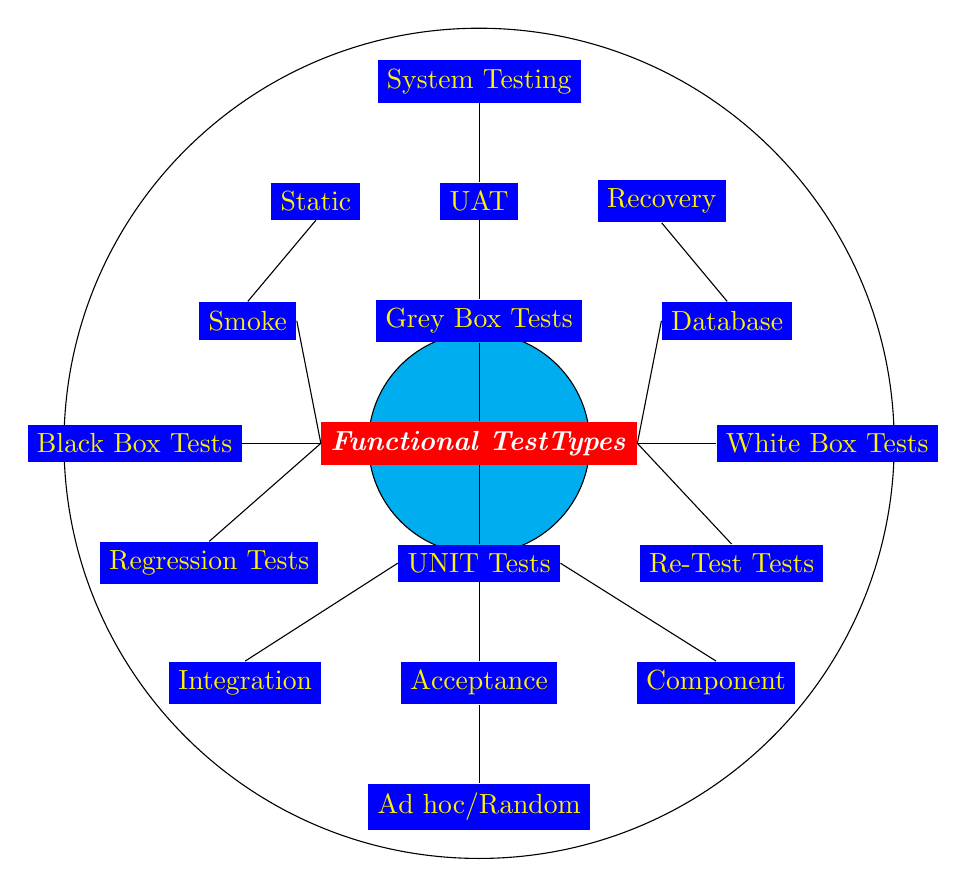
\begin{tikzpicture}
%% fun tests circle
\draw  [fill=white](0,0) circle  (150pt);
\draw  [fill=cyan](0,0) circle  (40pt);
%the nodes
\node [fill=red] (funCenter) { \color{white}\abbrhighcol{Functional Test \newline Types}};
\node [fill=blue,left=of funCenter] (funLeft) { \color{yellow}Black Box Tests};
\node [fill=blue,right=of funCenter] (funRight) { \color{yellow}White Box Tests};
\node [fill=blue,above=of funCenter] (funAbove) { \color{yellow}Grey Box Tests};
\node [fill=blue,below=of funCenter] (funBelow) { \color{yellow}UNIT Tests};
\node [fill=blue,left=of funBelow] (funBelowLeft) { \color{yellow}Regression Tests};
\node [fill=blue,right=of funBelow] (funBelowRight) { \color{yellow}Re-Test Tests};
\node [fill=blue,above=of funAbove] (funAboveAbove) { \color{yellow}UAT};
\node [fill=blue,left=of funAbove] (funAboveLeft) { \color{yellow}Smoke};
\node [fill=blue,right=of funAbove] (funAboveRight) { \color{yellow}Database};
\node [fill=blue,right=of funAboveAbove] (funAboveARight) {\color{yellow}Recovery};
\node [fill=blue,left=of funAboveAbove] (funAboveALeft) { \color{yellow}Static};
\node [fill=blue,below=of funBelow] (funBelowBelow) { \color{yellow}Acceptance};
\node [fill=blue,left=of funBelowBelow] (funBelowBLeft) { \color{yellow}Integration};
\node [fill=blue,right=of funBelowBelow] (funBelowBRight) { \color{yellow}Component};
\node [fill=blue,below=of funBelowBelow] (funBelowBBelow) { \color{yellow}Ad hoc/Random};
\node [fill=blue,above=of funAboveAbove] (funAboveAAbove) { \color{yellow}System Testing};
%drawings of lines
\draw[-] (funCenter.south) -- (funBelow.north);
\draw[-] (funCenter.north) -- (funAbove.south);

\draw[-] (funLeft.east) -- (funCenter.west);
\draw[-] (funCenter.east) -- (funRight.west);

\draw[-] (funCenter.east) -- (funAboveRight.west);
\draw[-] (funCenter.west) -- (funAboveLeft.east);

\draw[-] (funBelowLeft.north) -- (funCenter.west);
\draw[-] (funCenter.east) -- (funBelowRight.north);

\draw[-] (funBelowBelow.north) -- (funBelow.south);
\draw[-] (funAboveAbove.south) -- (funAbove.north);

\draw[-] (funAboveARight.south) -- (funAboveRight.north);
\draw[-] (funAboveALeft.south) -- (funAboveLeft.north);

\draw[-] (funBelowBLeft.north) -- (funBelow.west);
\draw[-] (funBelow.east) -- (funBelowBRight.north);

\draw[-] (funBelowBelow.south) -- (funBelowBBelow.north);
\draw[-] (funAboveAbove.north) -- (funAboveAAbove.south);

\end{tikzpicture}
\subsection{NON-Functional test-types overview (ALTERNATE)}
\begin{flushleft}
\end{flushleft}
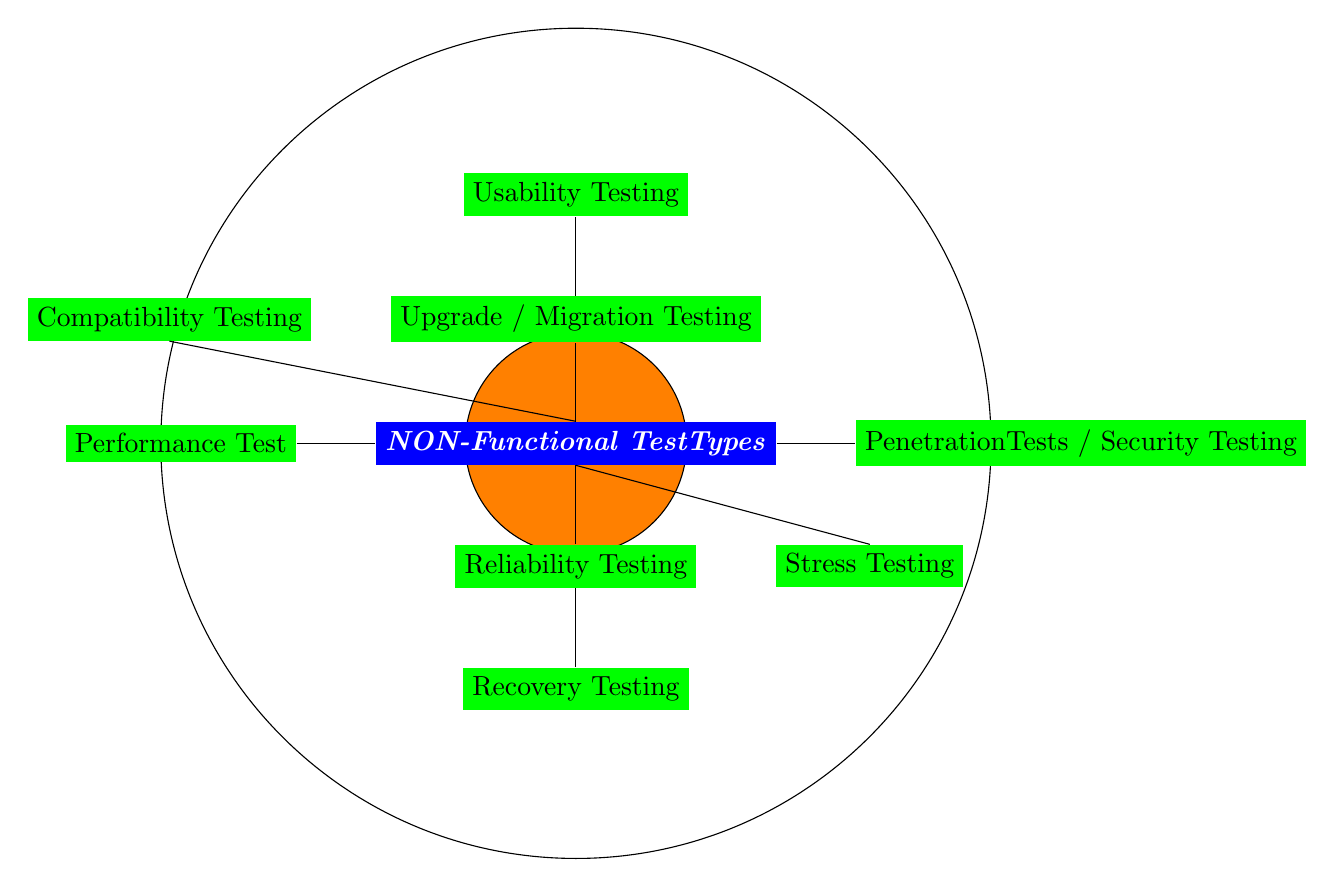
\begin{tikzpicture}
%% fun tests circle
\draw  [fill=white](0,0) circle  (150pt);
\draw  [fill=orange](0,0) circle  (40pt);
%the nodes
\node [fill=blue] (nfunCenter) { \color{white}\abbrhighcol{NON-Functional Test \newline Types}};
\node [fill=green,left=of nfunCenter] (nfunLeft) {Performance Test};
\node [fill=green,right=of nfunCenter] (nfunRight) {PenetrationTests / Security Testing};
\node [fill=green,above=of nfunCenter] (nfunAbove) {Upgrade / Migration Testing};
\node [fill=green,below=of nfunCenter] (nfunBelow) {Reliability Testing};
\node [fill=green,above=of nfunAbove] (nfunAboveAbove) {Usability Testing};
\node [fill=green,below=of nfunBelow] (nfunBelowBelow) {Recovery Testing};
\node [fill=green,left=of nfunAbove] (nfunAboveLeft) {Compatibility Testing};
\node [fill=green,right=of nfunBelow] (nfunBelowRight) {Stress Testing};
%drawings of lines
\draw[-] (nfunCenter.south) -- (nfunBelow.north);
\draw[-] (nfunCenter.north) -- (nfunAbove.south);

\draw[-] (nfunLeft.east) -- (nfunCenter.west);
\draw[-] (nfunCenter.east) -- (nfunRight.west);

\draw[-] (nfunCenter.south) -- (nfunBelowRight.north);
\draw[-] (nfunCenter.north) -- (nfunAboveLeft.south);

\draw[-] (nfunAbove.north) -- (nfunAboveAbove.south);
\draw[-] (nfunBelow.south) -- (nfunBelowBelow.north);
\end{tikzpicture}
\newpage
\section{Test types description}
\subsection{Functional Tests}
\begin{flushleft}
Functional tests have the focus on testing the functionality from outside for example calling services of an application in an application server. These tests MUST not know any implementation details but only in the case of the example the REST Service Interface or the Interface of whatever to test. The functional Tests are best placed in a functional tests project separated from the project where the development takes place. So they are clean separated and there is also not the danger for the one who develops them to have a deep look at the code. 
\end{flushleft}
\begin{enumerate}
\item{\abbrhighcol{UNIT Tests: }The focus of UNIT Tests is on the testing of the code units functions, methods of a class or a functional language in object oriented languages where we have private and public e have to look that we only test the public entries directly and the private entries as far as possible only indirect so that we do not break the language security mechanism of private access. The UNIT tests are written based on the knowledge of implementation details.}
\item{\abbrhighcol{Use Case Tests: }
The Use case tests are the next abstraction level. The focus is on testing the things in that units the use cases are defined in the projects specification. For example workflow for a banking transaction. These tests are sometimes automated and some projects need to do interactive / UI tests for that}
\item{\abbrhighcol{FeatureTests: }Features are new functionalities in a product or project the features can be a technical change with no interface change but they can also change the interfaces. This is the reason to test features in different ways. The one possibility only changes UNIT tests the other also changes for example rest services or the UI. Performance and regression tests have to be performed in both scenarios.A feature is part of a minor or major release.}
\item{\abbrhighcol{Black Box Tests: }Black Box Tests are tests of the functionality where the Tester who develops them only knows the interface, no matter if the interface is a library functionality a REST service or a UI interface}
\item{\abbrhighcol{Grey Box Tests: }Grey Box Tests are between Black Box Tests. The Tester knows some details about the implementation. For example he knows how the entry parameters are checked or he knows details about the structure used (module tree) for implementing a requirement. }
\item{\abbrhighcol{White Box Tests: }White Box Tests are tests where the Tester knows all the details about the implementation down to the last if condition or while loop.... }
\item{\abbrhighcol{Static Tests: }Static tests are a software testing practice that examines code and documentation without executing the program to find defects early in the development cycle. This is done by reviewing work products like source code, design documents, and requirements for inconsistencies, typos, security vulnerabilities, and deviations from standards. Static testing helps save time and money by catching and fixing errors before they escalate, improving code quality and maintainability. 
\begin{itemize}
\item{\abbrhighcol{What is tested: } Static testing can be applied to various work products, including requirements, design documents, and source code..}
\item{\abbrhighcol{What is found: } It can identify defects such as:
Syntax errors, dead code, and unused variables
Logic flaws and incorrect data/control flows
Security vulnerabilities like buffer overflows
Ambiguities, contradictions, and omissions in requirements
How it's performed: Static testing can be done manually through reviews and walkthroughs or automatically using tools called static analyzers.}
\end{itemize}}
\item{\abbrhighcol{System Tests: }A system test is a phase in the software development process where the complete, integrated software is tested to ensure it meets all specified requirements. It evaluates the system as a whole, focusing on how all the individual components work together, rather than testing them in isolation. This type of testing is typically conducted after unit and integration testing, and is often done using black-box testing methods to simulate a user's perspective.  }
\item{\abbrhighcol{Component Tests: }}
\item{\abbrhighcol{UAT Tests: }User Acceptance Tests are performed by the Users. The Users check how good a UI and how it is implemented fits their needss and if the look and feel is good. Since the projects and products are for the user these tests count as functional testing type}
\item{\abbrhighcol{Re-Tests: }Re-Tests are tests which are done if something was developed and tested . Imagine the tests shown up three errors so the tests checking these three conditions are re-executed after some fixes in the code}
\item{\abbrhighcol{Database Tests:} Database tests are tests for Database Schemas and database data structures e.g. in NoSQL, SQL databases. These data organisations are tested with the view on how good they support the functionality and the enhancements for the functionality.}. 
\item{\abbrhighcol{Recovery Tests: }Tests for a functional correct data recovery / failover tests are down there in the NON - Functional area.}
\item{\abbrhighcol{Integration Tests: }Integration tests are done to. see if the product or project is able to be integrated into the target system and its applications and infrastructure.}
\item{\abbrhighcol{Smoke Tests: }Tests for looking if one of the 'OK' paths is working for a functionality. For getting more complete also Exception tests are needed.}
\item{\abbrhighcol{Acceptance Tests: }In counter to the UAT these tests check the acceptance of the project or product against the specification of the functionality and if in each case the shortest way to do a task is realized}
\item{\abbrhighcol{Ad Hoc / Random Tests: } These tests are like the name tells us tests which are not in the usual testing scheme. Sometimes we have scenarios where the test by scheme is not sufficient so it is good to test things which are really unexpected e.g. Crazy inputs like prime numbers for a buffer size}
\item{\abbrhighcol{Regression Tests: }Regression tests are focused on checking if the functionality of the application works inn the same way after introducing features fixing bugs making changes (add ons) in the configuration and so on.}
\end{enumerate}
\subsection{NON-Functonal Tests}
\begin{flushleft}
\end{flushleft}
\begin{enumerate}
\item{\abbrhighcol{Performance Testing: }The focus of performance tests s on how fast a high amount of data or requests can be processed. To execute performance tests a realistic setup is necessary because if the tests run in a 'bubble' there is no way to distinct how performant the application really works in an environment like it is found at thee customers environment. In the best case all other applications driven by the customer run in parallel as it is in reality.  }
\item{\abbrhighcol{PenetrationTesting / Security Tests - Mostly Service Tests: }These tests are focused on checking the stability of the project in the way that requests to the software are placed in a way that the application can crash if it is not developed in a clean secure way. One of the possibilities is to send one or more requests which seem to be valid but which attack the application with incorrect data. Another possibility is that we send a mass of requests like in a DDOS Attack. There is no restriction in thinking about ways to put the whole thing out of order. Sometimes you have to think like the evil to get it secure.}
\item{\abbrhighcol{Upgrade / Migration Testing: }Some changes have an effect on external programs and data definitions like in a DBMS. These changes have to be upgraded automatically in best case. Here we have to decide if the Upgrade has to be possible from one release back or more releases back. What also needs a upgrade tests with a view on backward compatibility are Configurations either in the database e.g.: as CLOBS or XML, Properties or INI files}
\item{\abbrhighcol{Reliability Testing: }Checks if the system can perform consistently without failure over a specified period.}
\item{\abbrhighcol{Usability Testing: }Assesses how easy, efficient, and satisfying the system is for users to operate.They are defined in a way that they state if it is easily possible to use the functionality. Usability tests are in the best case not only done for the UI but also for the interfaces used by developers and administrators in this case we see the configuration strictly as part of the interface.}
\item{\abbrhighcol{Recovery Testing: }Verifies the system's ability to recover from crashes or failures.}
\item{\abbrhighcol{Compatibility Testing: }Verifies that the software works across different environments, browsers, or devices.}
\item{\abbrhighcol{Stress Testing: }Determines the breaking point of the system by overloading it beyond its normal capacity.}
\end{enumerate}

\subsection{Resume}
\begin{flushleft}
In general we can say that all these things have to be tested in different ways and that there is more than one possibility to test all these things. Some of the test scenarios are destined to be tested in a way that most of the parts are automated. This automation can be defined from the time point of check in to the point building a tested delivery. In the following chapters and sections we like to describe a way of automation which covers nearly all parts which has to be tested before delivery. 
\end{flushleft}
\chapter{Deep dive into test automation}
%% Next section
\section{Look at UNIT testing first}
\begin{flushleft}
The automation of Tests can take place on different levels of Test execution. At first take a look on test automation of \abbrhighcol{UNIT Tests}.\footnote{UNIT Tests are normally placed in the same project where the development takes place. The Tests are done on the programming language function level testig functions and / or classes and the implementation from the complete technical point of view}
The UNIT tests should be written by the developers coding the functions. There are two possibilities. Either the developer coding the function writes the UNIT tests during coding or the UNIT tests are written by the developer who does the code review which I think is very useful. I would prefer to do both things. First coding the function or write the UNIT test and code the function that it fits. After both things are written a code review should take place. Now the reviewer sees if there is something wrong in the code and / or if UNIT tests are missing and he can write further tests. In best case he writes tests which state if the errors he found are fixed. In most cases UNIT tests are per definition White Box Tests.
Here again our sort example. A typical simple UNIT test will be in Java with JUNIT:
\end{flushleft}
\begin{lstlisting}[language=Java]
   @Test
    public void testQuickSortSimple() {
        Integer[] arrayToSort = newArray();
        Integer[] arrayToSortComp = newArray();
        Arrays.<Integer>parallelSort(arrayToSortComp, new Comparator<Integer>() {
            @Override
            public int compare(Integer o1, Integer o2) {
                return o1.compareTo(o2);
            }
        });
        QBubbleMerge.quickSort(arrayToSort, ASC, 0, LAST_INDEX);
        assertThat(Arrays.compare(arrayToSort, arrayToSortComp), is(0));
        arrayToSort = newArray();
        arrayToSortComp = newArray();
        Arrays.<Integer>parallelSort(arrayToSortComp, new Comparator<Integer>() {
            @Override
            public int compare(Integer o1, Integer o2) {
                return o2.compareTo(o1);
            }
        });
        QBubbleMerge.quickSort(arrayToSort, DESC, 0, LAST_INDEX);
        assertThat(Arrays.compare(arrayToSort, arrayToSortComp), is(0));
    }
\end{lstlisting}
And in Python with the package unittest which is very similar:
\begin{lstlisting}[language=Python]
import unittest
import copy
from sort.algorithms.QBubbleMergeSort import QBubbleMergeSort
from sort.algorithms.SortData import SORT_DATA
from sort.algorithms.SortData import LAST_INDEX

class QBubbleMergeSortTest(unittest.TestCase):
    def test_quicksort_simple(self):
        toSortAsc = copy.deepcopy(SORT_DATA)
        toSortAsc.sort()
        toSortAscQuick = copy.deepcopy(SORT_DATA)
        QBubbleMergeSort.quickSort(toSortAscQuick, 0, LAST_INDEX)
        self.assertEqual(set(toSortAsc), set(toSortAscQuick))
\end{lstlisting}
\section{Functional Tests development in parallel}
\begin{flushleft}
Functional Tests are tests not only of one function in the technical sense but are tests to check if for example a defined REST request works in a proper way. The best way to define this tests is to have a separate test project. The functional tests are per definition black box tests. For the functional tests the technical definition of a REST request or client action ore something else is necessary. These tests are a abstraction level between UNIT and Use Case Tests.
\end{flushleft}
\section{Tests for Use Cases}
\begin{flushleft}
The tests for Use Cases is a test for a system / project / product requirement to check if the requirements defined by the customer are all implemented in a proper way. One example
will be a store of a document with signature like described above. To check if this works more than one functional tests may be executed in a transaction bracket.  
\end{flushleft}
\section{Setup / Build automated test environment}
\begin{flushleft}
To get automated tests in a structured designed way we have at first to take a look on which tools we need and use for getting the test process chained.
 Here is an example of tools and build automated tests with them this starts with the right ticket and task documentation tool. In our case we use JIRA. 
\end{flushleft}
\subsection{Example with toolchain}
\begin{flushleft}
% add more footnotes and open a references section
A toolchain is a set of software development tools used to build and otherwise develop software. Often, the tools are executed sequentially and form a pipeline such that the output of one tool is the input for the next. Sometimes the term is used for a set of related tools that are not necessarily executed sequentially. (Wikipedia)\newline
Our toolchain is a chain of tools we use for defining use cases and requirements which are broken down to tasks and sub-tasks for development. The development is done in an development environment like IntelliJ or Eclipse IDE and after being ready with a step it is committed to a Versioning Control System (VCS) like Bitbucket / GitHub (GIT). If the check in is done a Jenkins Build Job is triggered which builds the project / sub project. After this build the Jenkins in which the tests run is triggered so that the test run follows automatically. After that a deployment can be build. Either submitting the build in the Build Jenkins or we can use the test run afterwork to trigger the build of an assembly.\newline\abbrhighcol{The tools we use :}
\end{flushleft}
\begin{enumerate}
\item{JIRA: This tool is used to define and document the requirements, use cases, tasks , epics, tests, bugs and so on. It is the tool to define the project as well as the ticket system. Also teams and sprints can be defined in JIRA }
\item{Development Environment: E.G. IntelliJ... Tool for developing the project (Coding). }
\item{Versioning Control System: E.G. Bitbucket. Tool for versioning code and set up branches and releases -- the control system can be configured with JIRA so that check ins are tracked by task in JIRA }
\item{Build / Tests Tool: A tool like Jenkins can be used to set up build processes and test processes }
\item{Docker Containers can be used to set up systems and services for testing. Also the test run itself can be started in a separate docker}
\end{enumerate}
\newpage
\abbrhighcol{OVERVIEW - TOOLCHAIN}\newline\newline
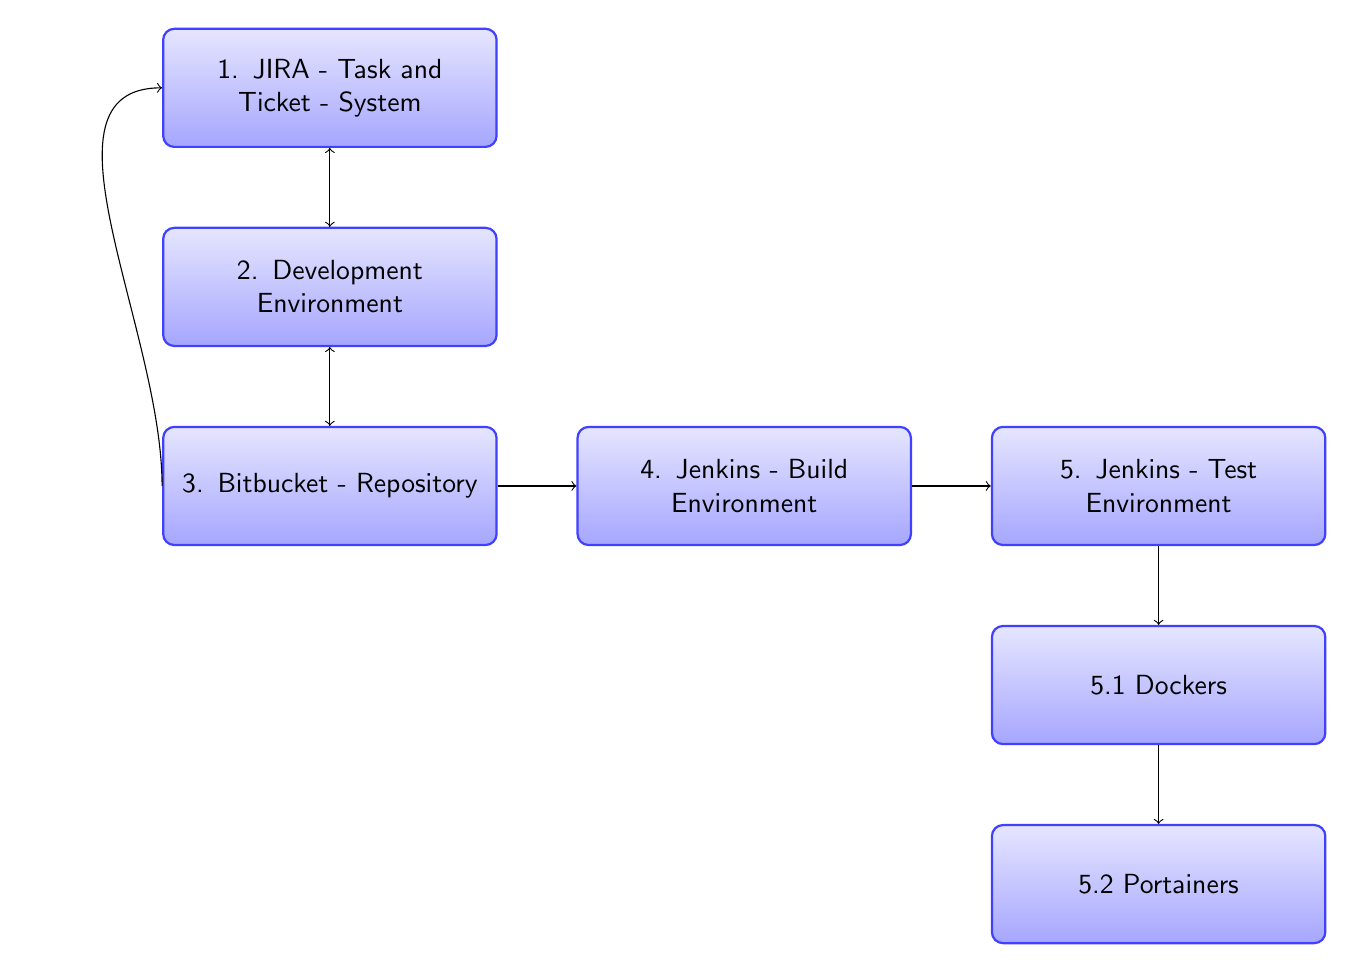
\begin{tikzpicture}
%the nodes
\node [simple module] (mA) {1. JIRA - Task and Ticket - System};
\node [simple module,below=of mA] (mA1) {2. Development Environment};
\node [simple module,below=of mA1] (mA2) {3. Bitbucket - Repository};
\node[simple module,right=of mA2](mB){4. Jenkins - Build Environment};
\node[simple module,right=of mB](mC){5. Jenkins - Test Environment}; 
\node[simple module,below=of mC](mD){5.1 Dockers}; 
\node[simple module,below=of mD](mE){5.2 Portainers}; 
%drawings of vectors
\draw[->] (mA.south) -- (mA1.north);
\draw[->] (mA1.north) -- (mA.south);
\draw[->] (mA1.south) -- (mA2.north);
\draw[->] (mA2.north) -- (mA1.south);
\draw[->] (mA2.west) .. controls +(up:20mm) and +(left:17mm) .. (mA.west);
\draw[->] (mA2.east) -- (mB.west);
\draw[->] (mB.east) -- (mC.west);
\draw[->] (mC.south) -- (mD.north);
\draw[->] (mD.south) -- (mE.north);
\end{tikzpicture}
\begin{flushleft}
Here we have a short overview on the whole tool-chain. Later after showing the different parts we will look how a typical workflow from Requirement to the Deploy will look like.
\end{flushleft}
\newpage
\abbrhighcol{1. JIRA-Task and Ticket-System}\newline\newline
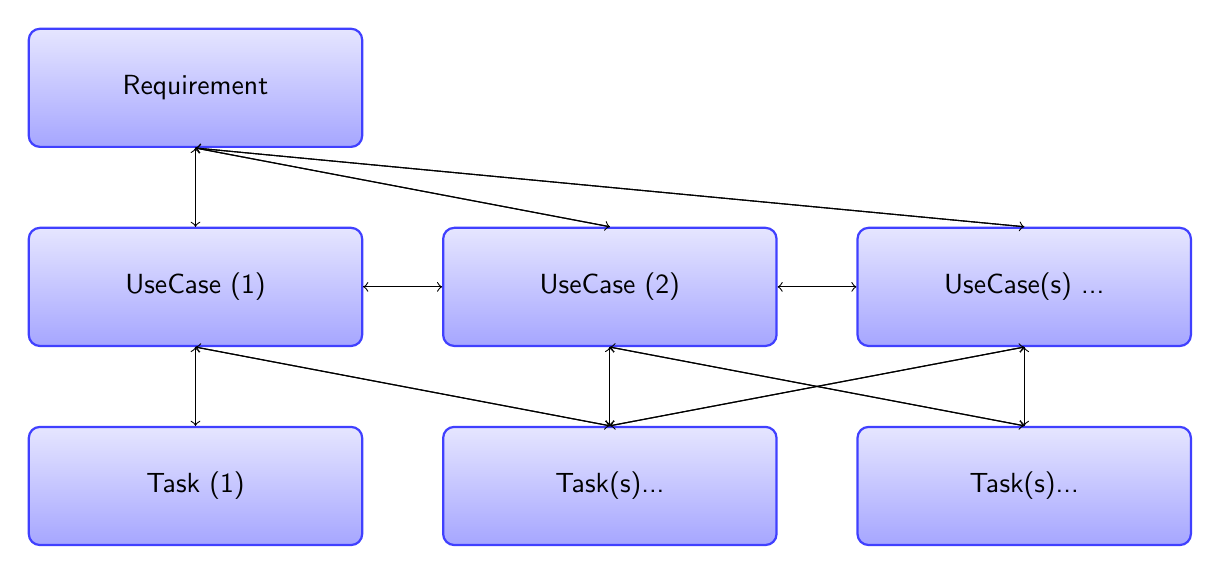
\begin{tikzpicture}
%the nodes
\node [simple module] (jA) {Requirement};
\node [simple module,below=of jA] (jB) {UseCase (1)};
\node [simple module,right=of jB] (jC) {UseCase (2)};
\node [simple module,right=of jC] (jD) {UseCase(s) ...};
\node [simple module,below=of jB] (jE) {Task (1)};
\node [simple module,right=of jE] (jF) {Task(s)...};
\node [simple module,right=of jF] (jG) {Task(s)...};
%drawings of vectors
\draw[->] (jA.south) -- (jB.north);
\draw[->] (jB.north) -- (jA.south);
\draw[->] (jA.south) -- (jC.north);
\draw[->] (jC.north) -- (jA.south);
\draw[->] (jA.south) -- (jD.north);
\draw[->] (jD.north) -- (jA.south);
\draw[->] (jB.east) -- (jC.west);
\draw[->] (jC.west) -- (jB.east);
\draw[->] (jC.east) -- (jD.west);
\draw[->] (jD.west) -- (jC.east);
\draw[->] (jB.south) -- (jE.north);
\draw[->] (jE.north) -- (jB.south);
\draw[->] (jB.south) -- (jF.north);
\draw[->] (jF.north) -- (jB.south);
\draw[->] (jC.south) -- (jF.north);
\draw[->] (jF.north) -- (jC.south);
\draw[->] (jC.south) -- (jG.north);
\draw[->] (jG.north) -- (jC.south);
\draw[->] (jD.south) -- (jF.north);
\draw[->] (jF.north) -- (jD.south);
\draw[->] (jD.south) -- (jG.north);
\draw[->] (jG.north) -- (jD.south);
\end{tikzpicture}\newline
\begin{flushleft}
We see here that in the end we have nearly something like a spider-net between the tasks and use cases. The reason is that there are many tasks which are the base for tasks which are specialised tasks for the use case xyz. 
\end{flushleft}
\abbrhighcol{2. Development Environment}\newline\newline
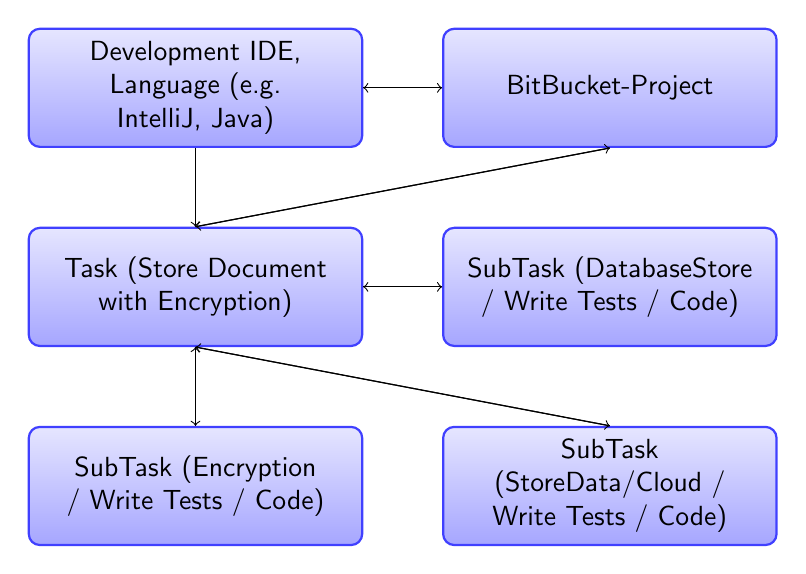
\begin{tikzpicture}
% the nodes
\node [simple module] (devA) {Development IDE, Language (e.g. IntelliJ, Java)};
\node [simple  module,below=of devA] (devB) {Task (Store Document with Encryption)};
\node [simple  module,below=of devB] (devC) {SubTask (Encryption / Write Tests / Code)};
\node [simple  module,right=of devB] (devD) {SubTask (DatabaseStore / Write Tests / Code)};
\node [simple  module,right=of devC] (devE) {SubTask (StoreData/Cloud / Write Tests / Code)};
\node [simple  module,right=of devA] (devF) {BitBucket-Project};
%drawings of vectors
\draw[->] (devA.south) -- (devB.north);
\draw[->] (devA.east) -- (devF.west);
\draw[->] (devF.west) -- (devA.east);
\draw[->] (devB.south) -- (devC.north);
\draw[->] (devC.north) -- (devB.south);
\draw[->] (devB.south) -- (devE.north);
\draw[->] (devE.north) -- (devB.south);
\draw[->] (devB.east) -- (devD.west);
\draw[->] (devD.west) -- (devB.east);
\draw[->] (devB.north) -- (devF.south);
\draw[->] (devF.south) -- (devB.north);
\end{tikzpicture}\newline
\begin{flushleft}
A typical workflow in the development environment will be that the developer gets a task and hast to break down the tasks in classes functions and configurations. The developer will choose one of the development tools which are allowed by the standard of the company or department. In this development environment the code is developed in a sandbox and later on the developer commits the code step by step to the version control system (e.g.: GIT) and then the development of the next function is done. A development environment should be choosed im a way that not only the pure coding is possible and that it supports some goodies e.g. Test Driven Development. In JIRA for example the developer can comment the task if necessary and he sees the output (what checked-in in GIT ) if he uses the feature of JIRA and BitBucket that the commits are grouped by task or defect. Normally a development Tool like IntelliJ supports all these things. 
\end{flushleft}
\newpage
\abbrhighcol{3. Bitbucket-Repository}\newline\newline
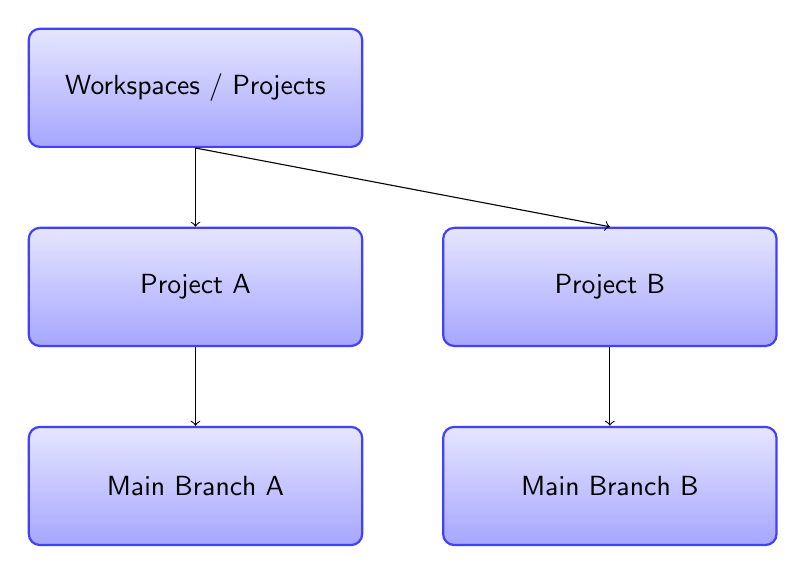
\begin{tikzpicture}
% the nodes
\node [simple module] (bbA){Workspaces / Projects};
\node [simple module,below=of bbA] (bbB){Project A};
\node [simple  module,right=of bbB] (bbC){Project B};
\node [simple  module,below=of bbB] (bbD){Main Branch A};
\node [simple  module,below=of bbC] (bbE){Main Branch B};
%drawings of vectors
\draw[->] (bbA.south) -- (bbB.north);
\draw[->] (bbA.south) -- (bbC.north);

\draw[->] (bbB.south) -- (bbD.north);
\draw[->] (bbC.south) -- (bbE.north);

\end{tikzpicture}\newline
\begin{flushleft}
The Bitbucket System holds GIT repositories. Each repository is a project or a sub-project which also may be dependent from one to the other. The projects can have a main Branch or several other branches which hold a specific step of development which is later on merged to the main branch. It is usual to make a code freeze for a release and after that run the major or minor release tests.
\end{flushleft}
\abbrhighcol{4. Jenkins-Build Environment}\newline\newline
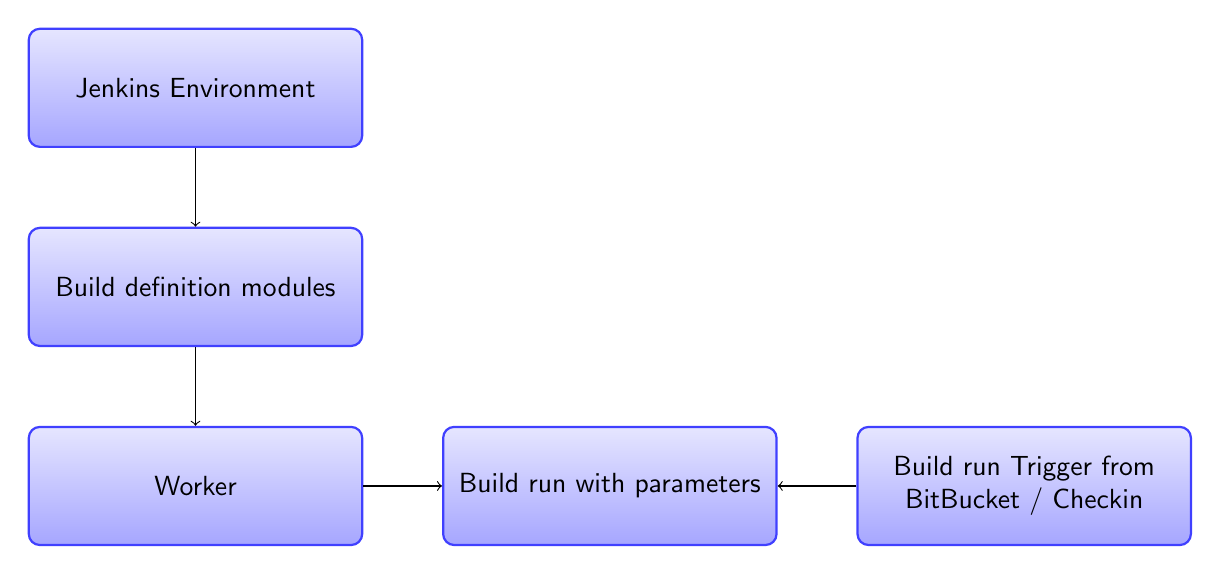
\begin{tikzpicture}
% the nodes
\node [simple module] (jbeA){Jenkins Environment};
\node [simple module,below=of jbeA] (jbeB){Build definition modules};
\node [simple  module,below=of jbeB] (jbeC){Worker};
\node [simple  module,right=of jbeC] (jbeD){Build run with parameters};
\node [simple  module,right=of jbeD] (jbeE){Build run Trigger from BitBucket / Checkin};
%drawings of vectors
\draw[->] (jbeA.south) -- (jbeB.north);
\draw[->] (jbeB.south) -- (jbeC.north);

\draw[->] (jbeC.east) -- (jbeD.west);

\draw[->] (jbeE.west) -- (jbeD.east);
\end{tikzpicture}\newline
\begin{flushleft}
The build environment is defined in a Jenkins instance. For each module or project is at least one build for the trunk defined and a release build. The build is triggered by a check in to BitBucket. After the build is successful the Tests in another Jenkins are triggered if defined. 
\end{flushleft}
\abbrhighcol{5. Jenkins-Test Environment}\newline\newline
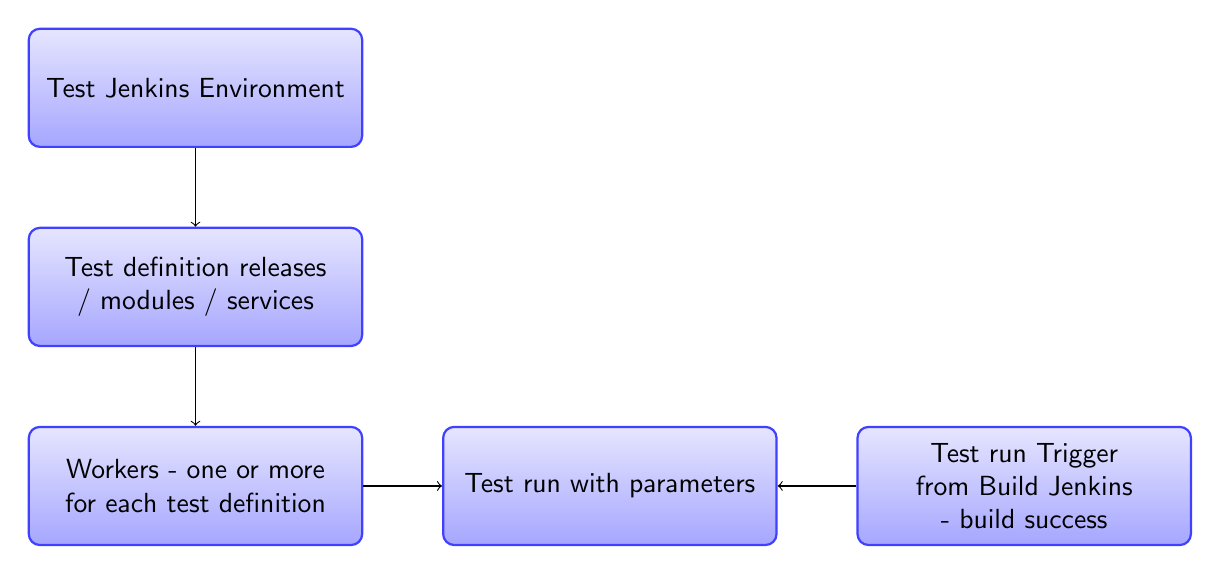
\begin{tikzpicture}
% the nodes
\node [simple module] (jteA){Test Jenkins Environment};
\node [simple module,below=of jteA] (jteB){Test definition releases / modules / services};
\node [simple  module,below=of jteB] (jteC){Workers - one or more for each test definition};
\node [simple  module,right=of jteC] (jteD){Test run with parameters};
\node [simple  module,right=of jteD] (jteE){Test run Trigger from Build Jenkins - build success};
%drawings of vectors
\draw[->] (jteA.south) -- (jteB.north);
\draw[->] (jteB.south) -- (jteC.north);

\draw[->] (jteC.east) -- (jteD.west);

\draw[->] (jteE.west) -- (jteD.east);
\end{tikzpicture}\newline
\begin{flushleft}
In the test part tests for many different projects or parts of projects are defined as test run. These test run definitions have 1-n workers assigned in these workers docker environments are established to run in Portainers. One of these docker environments is always the test run itself. The other belong to the application or service to be tested.
\end{flushleft}
\newpage
\subsection{The workflow in the tool-chain}
\chapter{Clean coding and project design as part of quality to make testing easier or possible}
\section{Rules for a clean project with proper testability}
\begin{flushleft}
One important thing to get a clean logic and a good quality is the design o the project in a way that the different parts/components can be tested separately as well as in a way that no mocking inside the project is necessary. Here some design patterns and rules as well as coding rules are very useful. First we like to take a look at the project design. 
\end{flushleft}
\subsection{How to design a application for getting a clean testable project}
\begin{flushleft}

\end{flushleft}
\subsection{A little view at coding styles necessary for testable code a few examples}
\begin{flushleft}
Here a little excursion regarding the coding style and how it can make testing of the code nearly impossible:
One important thing is to have a good style of coding doing conditional branches in the code:
For this have a look at Java\'s different styles of the switch statement:\newline
The output of the following functions is printed that way :
The thing is printed by;
\begin{lstlisting}[language=Java]
StringBuffer buffer = new StringBuffer()
                .append("Normal Simple: " + pureOldSwitchCase(SIMPLE))
                .append(" ; ").append("Normal Triple: " + pureOldSwitchCase(TRIPLE))
                .append(" ; ").append("Normal Double: " + pureOldSwitchCase(DOUBLE))
                .append(" ; ").append("Normal Fall through: " + pureOldSwitchCase(FALLTHROUGH))
                .append(" ; ").append("Normal default: " + pureOldSwitchCase(NONE))
                .append("\n\n")
                .append("With trap Simple: " + pureOldSwitchCaseWithTraps(SIMPLE))
                .append(" ; ").append("With trap Triple: " + pureOldSwitchCaseWithTraps(TRIPLE))
                .append(" ; ").append("With trap  Double: " + pureOldSwitchCaseWithTraps(DOUBLE))
                .append(" ; ").append("With trap  Fall through: " + pureOldSwitchCaseWithTraps(FALLTHROUGH))
                .append(" ; ").append("With trap  default: " + pureOldSwitchCaseWithTraps(NONE))
                .append("\n\n")
                .append("Upgraded Simple: " + upgradedOldSwitchCase(SIMPLE))
                .append(" ; ").append("Upgraded Triple: " + upgradedOldSwitchCase(TRIPLE))
                .append(" ; ").append("Upgraded Double: " + upgradedOldSwitchCase(DOUBLE))
                .append(" ; ").append("Upgraded Fall through: " + upgradedOldSwitchCase(FALLTHROUGH))
                .append(" ; ").append("Upgraded default: " + upgradedOldSwitchCase(NONE))
                .append("\n\n")
                .append("Upgraded Simple with traps: " + upgradedOldSwitchCaseWithTraps(SIMPLE))
                .append(" ; ").append("Upgraded Triple with traps: " + upgradedOldSwitchCaseWithTraps(TRIPLE))
                .append(" ; ").append("Upgraded Double with traps: " + upgradedOldSwitchCaseWithTraps(DOUBLE))
                .append(" ; ").append("Upgraded Fall through really fall: " + upgradedOldSwitchCaseWithTraps(FALLTHROUGH))
                .append(" ; ").append("Upgraded default with traps: " + upgradedOldSwitchCaseWithTraps(NONE))
                .append("\n\n")
                .append("new Simple Expr: " + newSwitchCaseExpr(SIMPLE))
                .append(" ; ").append("new Triple Expr: " + newSwitchCaseExpr(TRIPLE))
                .append(" ; ").append("new Double Expr: " + newSwitchCaseExpr(DOUBLE))
                .append(" ; ").append("new Fall through Expr: " + newSwitchCaseExpr(FALLTHROUGH))
                .append(" ; ").append("new default Expr: " + newSwitchCaseExpr(NONE))
                .append("\n\n");
        System.out.println(buffer);   
 \end{lstlisting}
\abbrhighcol{Let us first have a look at an old school nearly clean switch block}
\end{flushleft}
\begin{lstlisting}[language=Java]
 /**
     * In this function the break statements are set correctly and strict. 
     * Except the FALLTHROUGH: case that is no good style but in most cases acceptable.
     * @param rule the switch case criteria
     * @return the result for the selected case
     */ 
     public static Integer pureOldSwitchCase(ExecRules rule) {
        Integer x = 8;
        Integer y = 12;
        Integer result = 0;
        switch (rule) {
            case SIMPLE:
                result = x +3;
                break;
            case FALLTHROUGH: // this is seen as ok but no good style
                y *=9;
                result += 2 * y;   /*as you see here the break is missing the consequence is that the
                 execution falls through until the next break is set here before case TRIPLE: */ 
            case DOUBLE:
                result += y;
                break;   /*break sets the continuation to the statement after the switch actively*/
            case TRIPLE:
                result += 7;
                break;
            default:
                result += 3;
        }

        return result;
    }
\end{lstlisting}

The output calling it with all parameters will be:\newline
Normal Simple: 11; Normal Triple: 7 ; Normal Double: 12 ; Normal Fall through : 324 ; Normal default: 3\newline\newline
\abbrhighcol{Let us first have a look at an old school dirty coded switch block}
\begin{lstlisting}[language=Java]
/**
     * In this function the break statements are set wild or never. That kind of 
     * coding style leads to the fact that especially beginners cannot change the code so that all things work again.
     * There is no need to write such irritating code
     * Except the FALLTHROUGH: case that is no good style but in most cases acceptable.
     * @param rule the switch case criteria
     * @return the result for the selected case
     */
    public static Integer pureOldSwitchCaseWithTraps(ExecRules rule) {
        Integer x = 8;
        Integer y = 12;
        Integer result = 0;
        switch (rule) {
            case SIMPLE:
                result = x +3;
            case FALLTHROUGH:
                y *=9;
                result += 2 * y;
            case DOUBLE:
                result *= 2;
                result += y;
                break;
            case TRIPLE:
                result += 7;
            default:
                result += 3;
        }

        return result;
    }
\end{lstlisting}

The output calling it with all parameters will be:\newline
With trap Simple: 562 ; With trap Triple: 10 ; With trap  Double: 12 ; With trap  Fall through: 540 ; With trap  default: 3\newline\newline
\abbrhighcol{Let us first have a look at an new  clean coded switch block}
\begin{lstlisting}[language=Java]
 /**
     * Here we see the 'new' keyword yield with which a result is given back and which also, like break, sets the continuation
     * to go on after the switch. In this case here each branch ends with a yield so we have a clear and clean logic.
     * @param rule the switch parameter
     * @return the switch result
     */ public static Integer upgradedOldSwitchCase(ExecRules rule) {
        Integer x = 8;
        Integer y = 12;
        Integer result = 0;
        return switch (rule) {
            case SIMPLE:
                yield x +3;
            case FALLTHROUGH:
                yield y * 9;
            case DOUBLE:
                yield result + y;
                /*yield result = result + y; marked as unreachable */
            case TRIPLE:
                yield result + 7;
            default:
                yield result + 3;
        };
\end{lstlisting}

 The output calling it with all parameters will be:\newline
 Upgraded Simple: 11 ; Upgraded Triple: 7 ; Upgraded Double: 12 ; Upgraded Fall through: 108 ; Upgraded default: 3\newline\newline
\abbrhighcol{Now let us have a look at an new  tricky  coded switch block}
\begin{lstlisting}[language=Java]
 /**
     * Here one fallthrough takes place which is no clean coding since each branch should deliver
     * one defined return via yield
     * @param rule the switch value
     * @return the result of the switch 
     */
    public static Integer upgradedOldSwitchCaseWithTraps(ExecRules rule) {
        Integer x = 8;
        Integer y = 12;
        Integer result = 0;
        return switch (rule) {
            case SIMPLE:
                yield x +3;
            case FALLTHROUGH: // this is seen as ok but no good style
                y *=9;
                result += 2 * y;
            case DOUBLE:
                result *= 2;
                yield result + y;
            case TRIPLE:
                yield result + 7;
            default:
                yield result + 3;
        };

    }
\end{lstlisting}
 The output calling it with all parameters will be:\newline
 Upgraded Simple with traps: 11 ; Upgraded Triple with traps: 7 ; Upgraded Double with traps: 12 ; Upgraded Fall through really fall: 540 ; Upgraded default with traps: 3\newline\newline
 \abbrhighcol{Now let us see how the switch expression works here the continuations are impliit and so coding wit errors is more difficult}
\begin{lstlisting}[language=Java]
   /**
     * Here we see a switch EXPRESSION instead of a switch statement. All continuations are implicitly set
     * @param rule the switch parameter
     * @return the switch expression return
     */
    public static Integer newSwitchCaseExpr(ExecRules rule) {
        Integer x = 8;
        Integer y = 12;
        Integer result = 0;
        return switch (rule) {
            case SIMPLE ->
                    x + 3;   /*only THIS statement is executed and produces a  defined result */ 
             case FALLTHROUGH ->
                    y * 9;
            case DOUBLE -> /*only THIS statement is executed and produces a  defined result */
                    result + y;
            case TRIPLE ->   /*only THIS statement is executed and produces a  defined result */
                    result + 7;
            default ->.  /*only THIS statement is executed and produces a  defined result */
                    result + 3;
        };
    }
\end{lstlisting}  
The output calling it with all parameters will be:\newline
new Simple Expr: 11 ; new Triple Expr: 7 ; new Double Expr: 12 ; new Fall through Expr: 108 ; new default Expr: 3\newline\newline
\chapter{Further material}
\section{References}
\label{ref:references}
\begin{enumerate}
\item{\href{https://about.gitlab.com/ebook-ultimate-guide-ci-cd/variant/?utm_medium=cpc&utm_source=google&utm_campaign=eg_emea_dmp_x_x_en_gitlab_search_nb_singleappci-usecase_emea_broad&utm_content=eg_global_cmp_gated-content_depflex_en_guidecicd_x_x&&utm_term=cicd&_bt=740261293420&_bk=cicd&_bm=b&_bn=g&_bg=145507599496&gad_source=1&gad_campaignid=18463394777&gbraid=0AAAAADcJCbdc_52VE3ELeOTJbyqTR_PEd&gclid=CjwKCAiAlMHIBhAcEiwAZhZBUuxNCoQbO-WCuXyx0-26PE-PWqhcrsxolCDW-4gZq7TBt2eGK9hbvBoCgaYQAvD_BwE}{GITLAB CD/CI Guide and descriptions}}
\item{\href{https://solutionshub.epam.com/blog/post/the-difference-between-functional-and-non-functional-testing}{Definition of Functional and NON Functional Testing}}
\item{\href{https://solutionshub.epam.com/blog/post/regression-testing-test-io}{Regression Testing Tool and Description Regression Test IO}}  
\end{enumerate}
\end{document}